This research fits within the general topic of Explainable Agency~\cite{langley2017explainable}, whereby in order for people to trust autonomous agents, the latter must be able to explain their decisions and the reasoning that produced their choices.

% For example, explainable AI planning~\cite{fox2017explainable} 


Explanation of Constraint Satisfaction Problems (CSP) has been studied mostly in the context of over-constrained problems.
The goal then is to find a small set that conflict with each other.
The QuickXplain method \cite{junker2001quickxplain} for example uses a dichotomic approach that recursively partitions the constraints to find a minimal conflict set. Many other papers consider the same goal and search for explanations of over-constrainedness~\cite{leo2017debugging,zeighami2018towards}.
A minimal set of conflicting constraints is often called a \emph{minimal unsatisfiable subset} (MUS) or \emph{minimal unsatisfiable core} \cite{marques2010minimal}. Despite the fact that we do not (specifically) aim to explain overconstrained problems, our algorithms will internally also make use of MUS extraction methods.


% XAIP and queries
While explainability of constraint optimisation has received little attention so far, in the related field of \textit{planning}, there is an emerging subfield of \textit{eXplainable AI planning} (XAIP)~\cite{fox2017explainable}, which is concerned with building planning systems that can explain their own behaviour. This includes answering queries such as ``why did the system (not) make a certain decision?'', ``why is this the best decision?'', etc. In contrast to explainable machine learning research~\cite{guidotti2018survey}, in explainable planning one can make use of the explicit \textit{model-based representation} over which the reasoning happens. Likewise, we will make use of the constraint specification available to constraint solvers, more specifically typed first-order logic~\cite{atcl/Wittocx13}.

% 
% 
% We will use MUS extraction for finding a minimal explanation of an individual inference step.

Our work was inspired by the Holy Grail Challenge \cite{freuder2018progress} at the 2019 Constraint Programming conference (CP), which in turn has its roots in earlier work of E.~Freuder on inference-based explanations \cite{sqalli1996inference}.
In the latter, the authors investigate logic grid puzzles and develop a number of problem-specific inference rules that allow solving (most, but not all) such puzzles without search.
These inference rules are equipped with explanation templates such that each propagation event of an inference rule also has a templated explanation, and hence an explanation of the solution process is obtained.
We point out that the more complex inference rules (NCC and GNCC) are in fact inference rules over hard-coded combinations of (in)equality constraints.
In contrast, our proposed method works for any type of constraint and any combination of constraints, and automatically infers a minimal set of facts and constraints that explain an inference step, without using any problem-specific knowledge.
This powerful combination of constraints is able to automatically detect interesting consistency patterns that needed to be hand-coded in the Freuder's seminal work, but also in the solutions submitted by other
contenstants to the challenge \cite{escamocher2019solving}. %, who introduced a \emph{path consistency} inference rule which states that two entities cannot be linked in the solution to the puzzle if there exists another entity type such that for each element of the other type, one of the two entities cannot be linked to it \bart{Rephrase: clarify}.

\begin{figure}[ht]
    \centering
    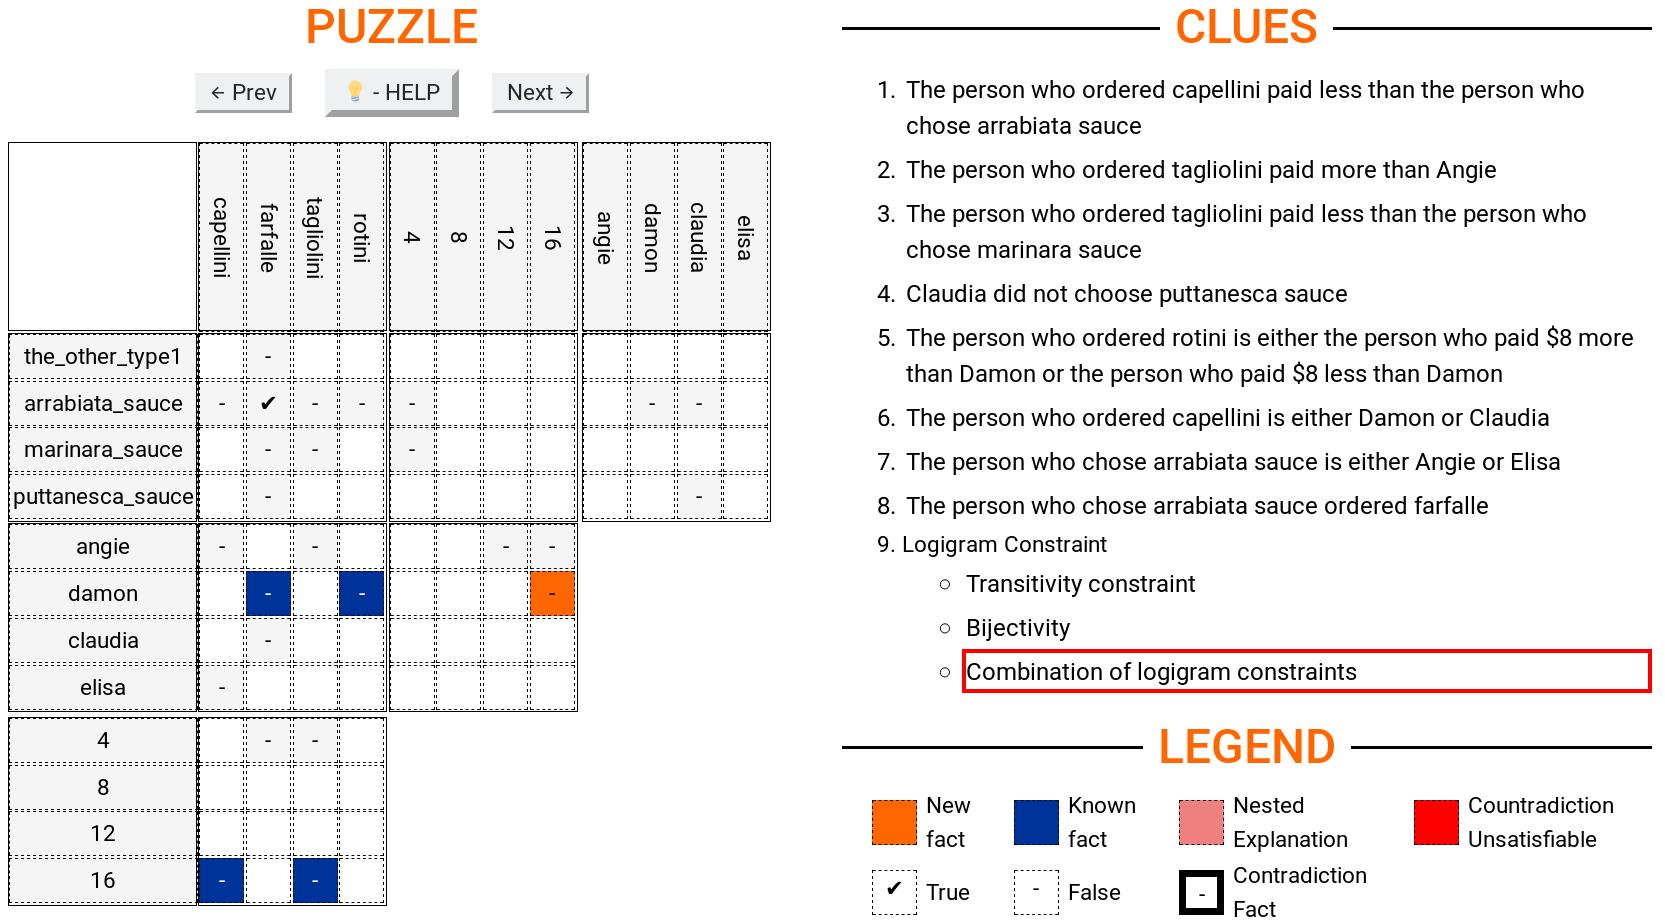
\includegraphics[width=0.7\linewidth]{figures/related_work.jpeg}
    \caption{Demonstration of explanation visualisation.}
    \label{fig:zebrascreen:path}
\end{figure}

Figure \ref{fig:zebrascreen:path} shows an example of a non-trivial explanation that our approach automatically generated, a combination of a so-called bijectivity and transitivity constraints, which was hard-coded as the special-purpose 'path consistency' pattern in earlier logic-grid specific work~\cite{sqalli1996inference}.
% \todo{add screenshot}


There is a rich literature on automated and interactive theorem proving, recently focussing on providing proofs that are understandable for humans \cite{Ganesalingam2017} and, e.g.,  on teaching humans -- using interaction with theorem provers -- how to craft mathematical proofs \cite{DBLP:conf/icml/YangD19}.
Our work fits into this line of research since our generated explanations can also be seen as proofs, but in the setting of finite-domain constraint solving.

Our approach also relates to the work of Belahcene et.\ al.~\cite{belahcene2017explaining} who --- in the context of decision-aiding --- aim to build incremental explanations using preference relations. In our case, this would correspond to preferring simple constraints to more complex combinations of constraints through a cost function.
